\subsection{The Plum Pudding Model}

There were numerous models that tried to tackle this problem and one of the first was proposed by Thompson in 1904 as the plum pudding model.
The first problem to grapple with was that electrons are negatively charged while the atoms themselves are electrically neutral.
To get around this, the plum pudding model suggests that  the electrons were suspended in a morass of positively charged particles
\footnote{Kind of like plums suspended in a pudding, hence the name of the model}
with the charge between the positive  and negative equalling out to 0.
Thomson believed that the mass was evenly distributed throughout the atom.

\begin{figure}[H]
  % https://en.m.wikipedia.org/wiki/File:Plum_pudding_atom.svg
  \centering
  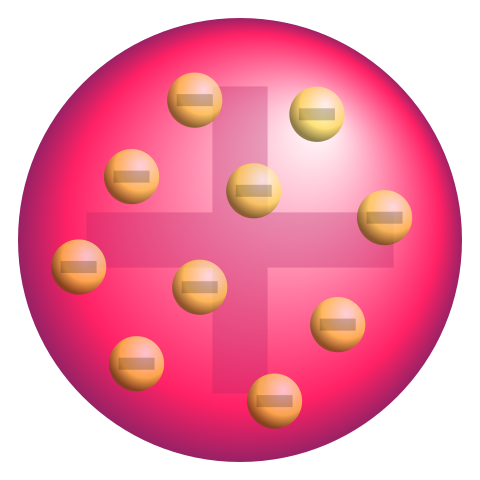
\includegraphics[width=100mm]{figures/plumPudding.png}
  \caption{Cartoon of plum pudding model}
  \label{plumPudding}
\end{figure}

The plum pudding model struggled to explain how these charged particles were so copacetic with each other despite being such small physical distances apart.
It was well known by then that opposite charges attract while alike charges repel.
It also failed to provide any explanation of the spectral lines observed in hydrogen.
Darker clouds were still on the horizon for Thomson's plum pudding model.
